\documentclass{standalone}
\usepackage{tikz}
\begin{document}
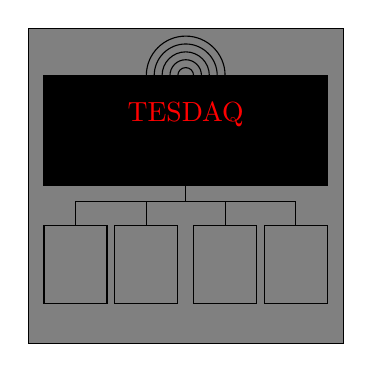
\begin{tikzpicture}[scale=2]
	\draw[fill=gray] (-1,1) rectangle (1,-1);
	\draw[fill=black] (-.9,0.7) rectangle (.9,0);
	\node[text=red,thick] (label) at (0,0.45) {TESDAQ};
	\foreach \r in {0,...,5}{
		\draw (0+0.05*\r,0.7) arc (0:180:0.05*\r);
		}
	\foreach \x in {-0.9, -0.45, 0.05, .5}{
		\draw (\x,-0.25) rectangle (\x+0.4,-0.75);
		\draw (\x+0.2,-0.25) -- (\x+0.2,-0.1) -- (0,-0.1) -- (0,0);5
		}
\end{tikzpicture}
\end{document}


